 %%	SECCION documentclass																									 %%	
%%---------------------------------------------------------------------------%%
\documentclass[a4paper]{report}

%%---------------------------------------------------------------------------%%
%%	SECCION usepackage																											 %%	
%%---------------------------------------------------------------------------%%
\usepackage{amsmath, amsthm}
\usepackage[spanish,activeacute]{babel}
\usepackage{caratula}
\usepackage{a4wide}
\usepackage{hyperref}
\usepackage{fancyhdr}
\usepackage{graphicx} % Para el logo magico!
\usepackage{amssymb}
\usepackage{amsmath}
\usepackage{float}
\usepackage[latin1]{inputenc}
%\usepackage [T1]{fontenc}
\usepackage[dvipsnames,usenames]{color}
\usepackage{amsfonts}
\usepackage{ulem}
%\usepackage{highlight}
\usepackage{fancybox}
%\usepackage{marvosym}
\usepackage{color}
\usepackage{lastpage}
\usepackage{lscape}
\usepackage{tabularx}
\usepackage{algorithmic}
\usepackage{algorithm}

%%---------------------------------------------------------------------------%%
%%	SECCION opciones																												 %%	
%%---------------------------------------------------------------------------%%
\parskip    = 11 pt
\headheight	= 13.1pt
\pagestyle	{fancy}
\definecolor{orange}{rgb}{1,0.5,0}

\addtolength{\headwidth}{1.0in}

\addtolength{\oddsidemargin}{-0.5in}
\addtolength{\textwidth}{1.0in}
\addtolength{\topmargin}{-0.5in}
\addtolength{\textheight}{0.7in}

%%---------------------------------------------------------------------------%%
%%	SECCION document	 %%	
%%---------------------------------------------------------------------------%%
\begin{document}
\renewcommand{\chaptername}{Parte }
\renewcommand{\algorithmicrequire}{\textcolor{blue}{\textbf{Requiere:}}}
\renewcommand{\algorithmicensure}{\textbf{Asegura:}}
\renewcommand{\algorithmicend}{\textbf{Fin}}
\renewcommand{\algorithmicif}{\textcolor{blue}{\textbf{Si}}}
\renewcommand{\algorithmicthen}{\textcolor{blue}{\textbf{entonces}}}
\renewcommand{\algorithmicelse}{\textcolor{red}{\textbf{Si no}}}
\renewcommand{\algorithmicelsif }{\textcolor{blue}{\textbf{Si no y}}}
\renewcommand{\algorithmicendif}{\textcolor{blue}{\textbf{Fin si}}}
\renewcommand{\algorithmicfor}{\textcolor{ForestGreen}{\textbf{Para}}}
\renewcommand{\algorithmicendfor}{\textcolor{ForestGreen}{\textbf{Fin para}}}
\renewcommand{\algorithmicwhile}{\textcolor{ForestGreen}{\textbf{Mientras}}}
\renewcommand{\algorithmicendwhile}{\textcolor{ForestGreen}{\textbf{Fin mientras}}}
\renewcommand{\algorithmicdo}{\textcolor{ForestGreen}{\textbf{hacer}}}
\renewcommand{\algorithmicreturn}{\textbf{Devolver}}
\floatname{algorithm}{Algoritmo}

%%---- Caratula -------------------------------------------------------------%%
\materia{Problemas, Algoritmos y Programaci�n (1er cuatrimestre de 2010)}
\titulo{Trabajo Pr�ctico A}

\integrante{Gonzalez, Emiliano}{426/06}{xjesse\_jamesx@hotmail.com}
\integrante{Gonzalez, Sergio}{481/06}{gonzalezsergio2003@yahoo.com.ar}
\integrante{Tleye, Sebastian}{732/05}{s\_tleye@yahoo.com.ar}
\resumen{
En el siguiente documento, se explicar�n las soluciones encontradas a los 4 problemas
planteados para esta entrega del trabajo pr�ctico, asi tambi�n como sus modelos y algoritmos utilizados para resolverlos. Para cada uno de estos adem�s, se determinar� y demostrar� su complejidad computacional expresada en funci�n de los parametros de entrada de cada uno de los
problemas.}

% TOC, usa estilos locos
\maketitle
\pagestyle{empty}
{
\fancypagestyle{plain}
    {
    \fancyhead{}
    \fancyfoot{}
    \renewcommand{\headrulewidth}{0.0pt}
    } % clear header and footer of plain page because of ToC
\tableofcontents
}

\newpage
% arreglos los estilos para el resto del documento, y
% reseteo los numeros de pagina para que queden bien
\pagenumbering{arabic}
\fancypagestyle{plain} {
    \fancyhead[LO]{Gonzalez, Gonzalez, Tleye}
    \fancyhead[C]{}
    \fancyhead[RO]{P\'agina \thepage\ de \pageref{LastPage}}
    \fancyfoot{}
    \renewcommand{\headrulewidth}{0.4pt}
}
\pagestyle{plain}

\newpage
\chapter{Problema 1}

\section{Edit Step Ladders}

\subsection{Enunciado}

Un $edit$ $step$ es una transformaci�n de una palabra $x$ en otra palabra $y$, tal que $x$ e $y$ son palabras en un diccionario de palabras y adem�s $x$ puede ser transformada en $y$ $agregando$, $borrando$ o $cambiando$ una letra. La transformaci�n de $dig$ a $dog$ o de $dog$ a $do$ son ambas $edit$ $steps$.

Un $edit$ $step$ $ladder$ es una secuencia ordenada alfab�ticamente $w_1$, $w_2$ ... $w_n$ tal que la transformaci�n de $w_i$ a $w_{i+1}$ es un $edit$ $step$ para todos los $i$ de 1 a n-1.

Se pide entonces, dado un diccionario de palabras, calcular el $edit$ $step$ $ladder$ mas largo.

\textbf{Input:}

El input consiste en un diccionario de palabras (en min�scula y ordenada alfab�ticamente) una por linea. Ninguna palabra tiene m�s de 16 letras y no hay mas de 25000 palabras en el diccionario.

\textbf{Output:}

El output consiste en un numero, que indica el $edit$ $step$ $ladder$ mas largo.

\textbf{Url:}

\href{http://uva.onlinejudge.org/index.php?option=com\_onlinejudge\&Itemid=8\&category=12\&page=show\_problem\&problem=970}{Problema de los edit step ladders}

\subsection{Soluci�n}
Para llegar a la soluci�n de este problema, se pensaron varios modelos y algoritmos. Algunos eran deficientes en cuanto a complejidad, tardando demasiado tiempo en resolver el problema y otros no lo resolv�an.

El algoritmo final, resuelve el problema en un tiempo razonable y por ende su complejidad es bastante buena. El mismo responde a un modelo iterativo, que depende de las palabras de entrada del problema y que va reutilizando datos que fueron calculados en pasos anteriores. Este m�todo utiliza el concepto de que cada informaci�n calculada anteriormente es �ptima, y por lo tanto para llegar a la soluci�n �ptima del valor actual, la misma se obtiene utilizando las soluciones optimas anteriores. Este concepto es muy importante y es el que define al m�todo de programaci�n din�mica, utilizado en este problema.

Comenzando entonces a describir el algoritmo creado para resolver el m�ximo edit step ladder de una lista de palabras, podemos decir que el mismo consta de cuatro grandes pasos:

\begin{enumerate}

\item El primero, es el de recorrer cada una de las palabras desde el principio hasta el final.
\item El segundo, se encarga de, dado una palabra actual ($P$), generar otras palabras que se consideren edit step de dicha $P$, es decir, que difieran de �sta en a lo sumo un caracter (ya sea quit�ndolo, agreg�ndolo, o modific�ndolo).
\item El tercer paso, utiliza las palabras generadas en el paso anterior y su funci�n es verificar si cada una de �stas, est� presente antes de $P$. Si alguna de �stas palabras es hallada, quiere decir que existe un edit step, por lo tanto, se puede agrandar en uno la distancia del step ladder de dicha palabra. En este paso, se utiliza lo calculado en pasos anteriores, es decir que cuando una palabra es hallada, la misma tiene asociado un valor que corresponde al mayor edit step ladder que termina en esa palabra. Por esta raz�n se ahorran c�lculos innecesarios, que adem�s ya fueron calculados anteriormente. Cabe aclarar que por cada palabra que es hallada, se verifica si se puede maximizar el edit step ladder hasta $P$, dicho de otra forma, se toma la palabra hallada que tenga mayor edit step ladder, de forma tal, que el valor asociado a la palabra actual $P$, sea el �ptimo. En este paso entra en juego el principio de optimalidad que se plantea en la programaci�n din�mica, ya que para asignarle el mejor step ladder que termina en la palabra actual $P$ (es decir el de mayor largo), el algoritmo se basa en decidir, cual es la palabra que maximiza su escalera y donde cada una de estas palabras tiene asociado con sigo, el mayor edit step ladder hasta ella (un valor �ptimo). Por esta raz�n, podemos decir que siempre que se tome el mayor valor dentro de las palabras que pueden ir de ellas a $P$, el valor de la palabra actual $P$ ser� �ptimo.
\item Por �ltimo, el cuarto paso consiste en verificar si el edit step ladder calculado para $P$, es el mas grande entre todos los que se calcularon anteriormente. Si esto es cierto, el valor de edit step ladder de $P$ pasa a ser el posible valor que se retornar� una vez que se finalice el recorrido de todas las palabras.
\end{enumerate}


Para dejar un poco m�s en claro, el funcionamiento del algoritmo de soluci�n, a continuaci�n se muestra la ecuaci�n de recurrencia asociada:

$maxStepLadders( N ) = \left\{ \begin{array}{lll}
0 & {\rm si \ } N = 0 \\
1 & {\rm si \ } N = 1 \\
1 + MAX_{1<= i <= N}( maxStepLocal( i ) ) & {\rm si \ } N > 1
\end{array}\right.
$

$maxStepLocal(i) = \left\{ \begin{array}{ll}
1 + max_{j \in posiblesStep(N)}(maxStepLocal(j)) & {\rm si \ } \exists(j, palabras [j] \in PosiblesStep(i)) \\
1 & {\rm sino \ }
\end{array}\right.
$

Como se puede observar, $maxStepLadders$ devuelve el resultado buscado, y en ella se puede ver de forma sobresaliente, que se efect�an los pasos $uno$ (recorrer las palabras) y $cuatro$ (quedarse con el mejor edit step ladder). En maxStepLocal, podemos observar que se llevan a cabo los pasos $dos$ (generar los posibles steps para una palabra) y $tres$ (seleccionar la que maximice el edit step ladder a la palabra actual).


\subsection{C�lculo de complejidad}

En �sta secci�n, demostraremos la complejidad computacional de la soluci�n creada. Para calcular dicha complejidad, utilizaremos el pseudoc�digo del algoritmo y describiremos cuales son los costos de realizar las operaciones involucradas en cada l�nea.

El pseudoc�digo es el siguiente:

\begin{algorithm}[H]
\caption{Calcula el step ladder de largo m�ximo}
\label{alg:algoritmo1b}
\begin{algorithmic}[1]
\PARAMS{cantidad de palabras}
\STATE inicializar los maximos step ladders de cada palabra en 1
\STATE inicializar maxLadder = 1
\FOR{cada palabra P}
	\STATE \COMMENT{borrado de letras}
	\STATE borrar de a un caracter por vez de P y buscar esta nueva palabra en las palabras anteriores a P
	\STATE si se encuentra actualizar el max step ladder de P
	\STATE \COMMENT{reemplazo de letras}
	\STATE reemplazar las letras de P de a una por vez por las letra del abecedario desde `a� hasta la letra a cambiar, formando $P'$
	\STATE buscar $P'$ en las palabras anteriores a P
	\STATE si se encuentra actualizar el max step ladder de P
	\STATE \COMMENT{agregado de letras}
	\STATE agregar letras de a una por vez en cada posicion de P formando $P'$
	\STATE buscar $P'$ en las palabras anteriores a P
	\STATE si se encuentra actualizar el max step ladder de P
	\STATE actualizar maxLadder
\ENDFOR
\RETURN maxLadder
\end{algorithmic}
\end{algorithm}

Como primer paso, definimos algunas cuestiones con respecto respecto a los simbolos que se utilizar�n para demostrar la complejidad del algoritmo.

El enunciado menciona que, se recibir� una lista de palabras ordenadas alfabeticamente. Estas palabras son la entrada del problema, y de �sta entrada depende nuestra soluci�n, por este motivo vamos a tomar a la cantidad de palabras como parametro para calcular la complejidad. A dicha cantidad la definiremos como $N$, y de �sta forma se har� referencia a la cantidad de palabras de entrada en los proximos p�rrafos.

Adem�s se menciona, que el largo de las palabras se encuentra acotada. Si bien dicho valor no va a resultar importante en la complejidad final (ya que la misma se expresar� con el valor de una funci�n que crezca asintoticamente igual) lo usaremos en el calculo intermedio y dicho valor lo denominaremos $L$. Si bien el largo de las palabras no son iguales, podemos decir que $L$ se corresponde con el largo de la palabra mas larga dentro de la lista.

Las primeras dos lineas son inicializaciones de variables, donde en la linea 1 se inicializa un arreglo que tiene tantas posiciones como palabras en el arreglo de palabras (que tiene costo lineal con respecto a la cantidad de palabras). La segunda es una asignacion normal a una variable (de costo constante). De las observaciones anteriores podemos decir que hasta la linea 2, existe una complejidad lineal en funci�n de la entrada ($N$).

En la linea 3 comienza un ciclo de tipo $for$ que termina en la linea 16, aqu� se recorren todas las palabras de la entrada (se corresponde con el paso n�mero $1$ en la introducci�n de la soluci�n), dicho ciclo entonces se har� tantas veces como palabras haya en la entrada, es decir $N$ veces.

En las partes comentadas como �borrado de letras�, �reemplazo de letras� y �agregado de letras� se efectua el paso n�mero $2$, que consiste en generar los posibles edit step de la palabra actual. Las tres partes son similares en cuanto a pasos que se realizan para obtener los posibles edit step. La Idea principal en las tres partes consiste en recorrer cada posici�n de la palabra y realizar una operaci�n (ya sea para modificar, agregar o quitar una letra) y luego ver si la nueva palabra obtenida se encuentra en la lista de palabras que est�n antes de $P$. Recorrer cada posici�n de una palabra queda en funci�n del largo de la palabra ($L$). Como la lista de palabras se encuentra ordenada alfabeticamente, ver si cada nueva palabra generada est� dentro de la lista antes de $P$ se puede saber realizando un busqueda binaria, que queda en funci�n del logaritmo de la cantidad de palabras recorridas ($log_2(K)$, donde $K$ es la cantidad de palabras ya recorridas).

Con lo explicado anteriormente podemos ver que por cada ciclo del $for$ principal, se realizan 3 modificaciones de la palabra P, donde en cada una se recorre posicion por posicion de P y se busca en las palabras anteriores. Luego podemos decir que hacer un ciclo esta en funcion de hacer 3 veces el recorrido letra por letra y por cada una de ellas hacer una busqueda, que resultan en un costo de $3*L*log_2(K)$ (donde $K$ es la cantidad de palabras ya recorrida). Luego esto se realiza $N$ veces, entonces nos queda algo como lo siguiente:

\medskip
\centerline{ $3*L*log_2(1) + 3*L*log_2(2) + ... + 3*L*log_2(N)$ }

Dicha cuenta la podemos acotar superiormente, considerando que cada valor dentro de los logaritmos, son menores o iguales a $N$. Lo que resulta en lo siguiente:

\centerline{ $3*L*log_2(1) + 3*L*log_2(2) + ... + 3*L*log_2(N) {\rm  \ } \le {\rm  \ } 
3*L*log_2(N) + 3*L*log_2(N) + ... + 3*L*log_2(N) $}

\centerline{=}

\centerline{$3*L*N*log_2(N)$}

A su vez, $L$ puede ser acotado superiormente por $16$, lo que nos dar�a que la complejidad estar�a en funci�n de $48*N*log_2(N)$. Teniendo en cuenta el orden asintotico de esta complejidad, podemos despreciar las constantes y finalmente decir, que el algoritmo de soluci�n esta en el orden de:

\medskip
\centerline{$O(N*log_2(N))$}
\clearpage

\newpage
\chapter{Problema 2}

\section{Little Bishops}

Un alfil es una pieza utilizada en el juego de ajedrez el cual es jugado en una tabla con grillas cuadradas. Un alfil puede moverse solamente de forma diagonal desde su posici�n actual, y dos alfiles se atacan si uno de ellos est� en el camino del otro. En la siguiente figura, los cuadrados negros representan los lugares alcanzables por el alfil $B_1$ desde su posici�n actual. La figura tambi�n muestra que los alfiles $B_1$ y $B_2$ est�n en posiciones de ataque, pero $B_1$ y $B_3$ no. $B_2$ y $B_3$ tampoco se atacan.

\begin{figure}[H]
\centering
\label{ej2_tableroEnunciado}
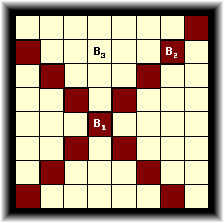
\includegraphics[scale=0.5]{./graficos/ej2/tableroEnunciado.jpg}
\end{figure}

Ahora, dados dos n�meros \textbf{n} y \textbf{k}, su deber es determinar la cantidad de formas en que uno puede ubicar $k$ alfiles en un tablero de ajedrez de $n � n$, de forma tal que ningun par de ellos se atacan.
 
\textbf{Entrada:}

El archivo de entrada puede contener m�ltiples casos de test. Cada test ocupa una l�nea en el archivo de entrada y contiene dos enteros \textbf{n} $(1 \le n \le 8)$ y \textbf{k} $(0 \le k \le n^2)$. 

Un caso de test que contiene dos ceros para n y k finaliza la entrada y no necesitar� procesar esta particular entrada.
 
\textbf{Salida:}

Para cada caso de test en la entrada imprimir una l�nea conteniendo el n�mero total de formas en la cual uno puede ubicar la cantidad de alfiles dada en un tablero de ajedrez del tama�o dado tal que ningun par de ellos se atacan. Puede asumir que este n�mero ser� menor a $10^{15}$.

\textbf{Url:}

\href{http://uva.onlinejudge.org/index.php?option=com\_onlinejudge\&Itemid=8\&category=10\&page=show\_problem\&problem=802}{Problema de Little Bishops}

\subsection{Soluci�n}

\clearpage

\newpage
\chapter{Problema 3}

\section{Distinct Subsequences}

Una subsecuencia de una secuencia dada es la secuencia con algunos elementos (posiblemente ninguno) faltantes. Formalmente, dada una secuencia $X = x_1, x_2, ..., x_m$, otra secuencia $Z = z_1, z_2, ..., z_k$ es una subsecuencia de X si existe una secuencia estrictamente creciente $< i_1, i_2, ..., i_k >$ de �ndices de X tal que para todo $j = 1, 2, ..., k$ tenemos $x_{i_j} = z_j$. Por ejemplo, $Z = bcdb$ es una subsecuencia de $X = abcbdab$ con su correspondiente secuencia de indices \verb|< 2, 3, 5, 7 >|.

Escribir un programa tal que cuente el n�mero de subsecuencias Z de X tal que cada una de ellas tiene una correspondiente subsecuencia de indices distinta.

\textbf{Entrada:}

La primer l�nea del input contiene un entero N indicando la cantidad de casos de test que siguen.

La primer linea de cada caso de test contiene una cadena X de una longitud no mayor a 10000, compuesta enteramente de caracteres del alfabeto en min�scula. La segunda l�nea contiene otra cadena Z de longitud no mayor a 100, y tambi�n compuesta solamente de caracteres del alfabeto en min�scula. Se asegura que ni Z ni ningun prefijo o sufijo del mismo tendr� m�s de $10^{100}$ distintas ocurrencias en X como subsecuencia.

\textbf{Salida:}

Para cada caso de test de la entrada, debe haber una salida correspondiente al numero de ocurrencias de Z en X como subsecuencia. La salida de cada caso de test de entrada debe hacerse en l�neas separadas.

\textbf{Url:}

\href{http://uva.onlinejudge.org/index.php?option=com\_onlinejudge\&Itemid=8\&category=12\&page=show\_problem\&problem=1010}{Problema de Distinct Subsequences}

\subsection{Soluci�n}

La soluci�n al problema resulta ser iterativa sobre los caracteres de la palabra $X$ y de la palabra $Z$ y b�sicamente se divide en 2 etapas:

\begin{itemize}
\item Paso 1: consiste en recorrer la secuencia $X$ en busca de caracteres que coincidan con alguno de los caracteres en la subsecuencia $Z$. Dicho recorrido se realiza de fin a principio, y la raz�n para hacerlo de esta forma es que se pueden ir contando la cantidad de veces que se puede formar parte de $Z$ desde la ubicaci�n actual de $X$ hasta el final de la misma. Esta idea la veremos un poco mas adelante con un ejemplo.
\item Paso 2: una vez encontrado un caracter de $X$ que coincida con alguno dentro de $Z$ (llam�moslo $C$), el paso 2 se encarga de contar la cantidad de veces que se puede formar la sub palabra dentro de $Z$ que comience en $C$ y termine en el final de $Z$. Para hacer esto se tienen que tener en cuenta las letras que le siguen a $C$ en $Z$ y que hayan aparecido en $X$ en iteraciones anteriores (recordar que las iteraciones se realizan de fin a principio). La idea detr�s de esto consiste en ver cuantas veces se puede formar la sub palabra comenzando en $C$ con las letras que ya se recorrieron.
\end{itemize}

Una vez descriptos los dos pasos b�sicos que realiza el algoritmo para resolver el problema, veremos un poco mas en detalle el paso 2, para explicar mejor como es que se hace para determinar cuantas veces se puede generar la sub palabra dentro de $Z$ y que comience en el caracter $C$ (que recordemos es el que coincide con el caracter actual en la iteraci�n sobre $X$). El m�todo consiste en asociar cada letra de $Z$ con un n�mero, donde �ste n�mero representar� la cantidad de veces que se puede formar la sub palabra que comience desde cada uno de los caracteres de $Z$ hasta el final de $Z$. Teniendo esto, por cada caracter que se encuentre en $X$ y que este contenido en $Z$, dicho caracter tendr� asociado la cantidad de veces que que se puede formar la sub secuencia comenzando en �l, que resulta ser la cantidad que ya se tenia registrada anteriormente, pero sum�ndole ahora, la cantidad de veces que se puede generar la sub palabra que comienza con la letra inmediata siguiente. Esto se puede ver que es sensato de pensar, ya que si no se puede generar ninguna sub palabra desde el caracter inmediato siguiente a $C$, tampoco se podr� generar ninguna desde $C$ y si en cambio se puede generar alguna sub palabra desde el inmediato siguiente a $C$, entonces se pueden generar tantas subpalabras desde $C$ como haya desde el caracter inmediato siguiente. Para terminar de cerrar la idea veremos un ejemplo donde se aplica el paso 2.

Veremos como funciona el paso 2 cuando se pueden generar sub palabras desde el caracter inmediato siguiente a $C$. Entonces para el siguiente ejemplo supongamos que se tiene una palabra $Z$ = �bit�, y supongamos que se estuvo recorriendo $X$ que tiene ciertas palabras. Hasta el momento sabemos que se puede generar una sola vez la subsecuencia de $Z$ = �it�, ya que se encontr� primero una �t� y luego una �i� durante el recorrido de $X$, y entonces se hayan 3 �b�s dentro de $X$.

\begin{figure}[H]
\centering
\subfigure[inicio, se tiene que ya aparecio �it�, donde primero aparecio �t� y luego �i�(notar que si la aparicion hubiese sido al rev�z, no se hubiese podido formar �it�), por este motivo �i� tiene asociado un 1, ya que cuando apareci�, sum� lo que tenia la letra inmediata siguiente �t�]{
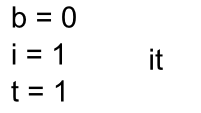
\includegraphics[scale=0.5]{./graficos/ej3/paso0.png}} \hspace{0.5in} 
\subfigure[llega una �b�, entonces existe una sola forma de formar �bit�, que es con la �nica forma de hacer �it�, por lo tanto se suma 1 al valor que se tenia en �b� (que es la cantidad de formas de formar �bit�)]{
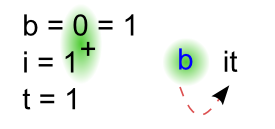
\includegraphics[scale=0.5]{./graficos/ej3/paso1.png} }\hspace{0.5in} 
\subfigure[llega la segunda �b� y nuevamente existe solo una forma de formar �bit� con dicha letra, pero tambi�n se podia formar con la anterior �b� que hab�a llegado, por ende al valor que se ten�a en �b� (valor 1) se le suma la cantidad de formas de formar �it�, que es la cantidad de veces que se puede formar �bit� con la �b� actual]{
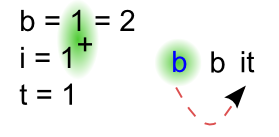
\includegraphics[scale=0.5]{./graficos/ej3/paso2.png}} \hspace{0.5in} 
\subfigure[llega la tercera �b�, y aqu� pasa lo mismo con los casos anteriores]{
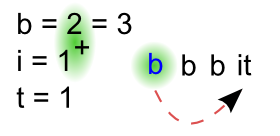
\includegraphics[scale=0.5]{./graficos/ej3/paso3.png}} \hspace{0.5in} 
\caption{resoluci�n para el caso en donde se puede generar la sub palabra �bit�}
\setcounter{subfigure}{0}
\end{figure}

Para un caso en donde no se pueda generar alguna sub palabra, queda claro que la letra inmediata siguiente tendr� valor cero, lo que significa que no se puede generar ninguna subpalabra que comience en dicha letra y termine en el final de $Z$. A modo de ejemplo de este caso, veamos que pasa si ahora en $X$ se encuentra primero �t� pero no se encuentra �i� y llegan 2 �b�s.

\begin{figure}[H]
\centering
\subfigure[inicio, se tiene que ya aparecio �t�, por este motivo �i� tiene asociado un 0 ya que no apareci� ninguna �i� para intentar formar �it�]{
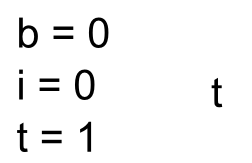
\includegraphics[scale=0.5]{./graficos/ej3/paso0ej2.png}} \hspace{0.5in} 
\subfigure[llega una �b�, entonces no existe forma de formar �bit�, ya que no ha llegado una �i�, por este motivo, la cantidad de veces que se puede formar �bit� es la misma para formar �it�, y que resulta ser 0, este es el valor que quedar� en �b�)]{
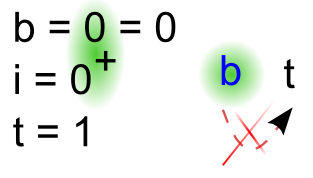
\includegraphics[scale=0.5]{./graficos/ej3/paso1ej2.png} }\hspace{0.5in} 
\subfigure[llega la segunda �b� y nuevamente no existe forma de formar �bit� con dicha letra]{
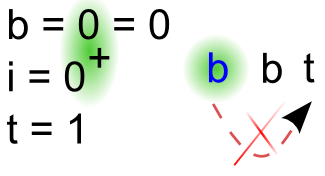
\includegraphics[scale=0.5]{./graficos/ej3/paso2ej2.png}} \hspace{0.5in} 
\caption{resoluci�n para el caso en donde se puede generar la sub palabra �bit�}
\setcounter{subfigure}{0}
\end{figure}

Como se puede observar, cada letra de $Z$ tiene asociado el valor que representa a la mayor cantidad de palabras que se pueden generar a partir de ella. De esta observaci�n podemos decir entonces que cada valor asociado a las letras de $Z$ es �ptimo respecto a dicha cantidad. Y entonces el c�lculo que resulta de sumar el valor actual con el valor de la letra inmediata siguiente, resulta en un valor �ptimo tambi�n, ya que se est� seguro que no existen mas formas de generar la misma palabra. De esta manera, si vemos al problema como uno de programaci�n din�mica podemos decir que el principio de �ptimalidad se cumple en esta parte.

Por otro lado podemos decir que, el valor a devolver como soluci�n del problema, ser� el valor que se encuentre en la primer letra de $Z$, ya que este indicar� la cantidad de veces que se puede formar $Z$ en $X$.

\subsection{Detalles de implementaci�n}

Este problema se destaca particularmente de los dem�s debido a que los n�meros (enteros) crecen r�pidamente, hasta tener cientos de d�gitos. Esto es as� debido a la cantidad de distintas ocurrencias de $Z$ en $X$, que como lo indica el enunciado, puede llegar a un orden de $10^{100}$. Los enteros en C++ tienen como m�ximo 8 bytes, es decir su m�ximo valor es $2^{64}$, o sea que no llega al orden de $10^{20}$, por lo tanto esto nos presenta un nuevo problema, el de no poder contar la cantidad de subsecuencias si el n�mero de ellas excede $2^{64}$. Para esto se cre� una clase llamada $VeryLongUnsignedInt$, que representa enteros de una cantidad infinita de d�gitos. Con esta implementaci�n adicional se pudo contar entonces las sub secuencias que se encontraban y devolver el resultado correcto.

La estructura interna de dicha clase, consiste en un arreglo de enteros sin signo del tipo $unsigned$ $long$ $long$ $int$, donde se va almacenando el n�mero de cifras arbitrarias. Cada operaci�n del tipo $+=$ que recibe 2 n�meros de este tipo, realiza un recorrido de cada una de las posiciones de los mismos a la par, y cuando sea necesario, asigna los carrys correspondientes. El valor l�mite antes de realizar un carry es de $1000000000$, por lo tanto al realizar las sumas de cada uno de los pares de n�meros, si el resultado excede dicho valor, se calcula el valor que quedar� en esa posici�n y el valor que ser� pasado a la posici�n siguiente (valor que representa carry). Con esta implementaci�n, a lo sumo se utilizan 9 elementos en el arreglo de un $VeryLongUnsignedInt$, ya que esta cantidad es la necesaria para representar $10^{100}$, que es el m�ximo numero de subsecuencias que puede haber.

\subsection{C�lculo de complejidad}

A continuaci�n se calcular� la complejidad del algortimo que calcula la soluci�n. Se har� en base a un pseudoc�digo que representa la funci�n resolver que dado una secuencia y una subsecuencia, calcula el numero de veces que dicha subsecuencia se encuentra dentro de la secuencia.

\begin{algorithm}[H]
\caption{Calcula la cantidad de ocurrencias de una subsecuencia en una secuencia}
\label{alg:algoritmo1b}
\begin{algorithmic}[1]
\PARAMS{Secuencia, Subsecuencia}
\STATE inicializar las Combinaciones para cada letra de la subsecuencia en 0
\FOR{cada caracter C de la secuencia de fin a principio}
	\FOR{cada caracter CSub de la subsecuencia tal que CSub $=$ C}
		\IF{CSub es el �ltimo caracter de la Subsecuencia}
			\STATE $Combinaciones_{longSubsec - 1}$ $\leftarrow$ $Combinaciones_{longSubsec - 1} + 1$
		\ELSE
			\STATE i $\leftarrow$ indice del caracter CSub de la subsecuencia
			\STATE $Combinaciones_i$ $\leftarrow$ $Combinaciones_{i + 1}$
		\ENDIF
	\ENDFOR
\ENDFOR
\RETURN $Combinaciones_0$
\end{algorithmic}
\end{algorithm}

Como la funci�n recibe dos par�metros, la complejidad de dicha funci�n queda determinada entonces por estos. Sea entonces $N$ el largo de la secuencia recibida y $L$ el largo de la subsecuencia, con �stos valores se demostrar� la complejidad.

La primer linea inicializa el vector donde se alojar�n los valores relacionados con cada letra de la subsecuencia como se coment� previamente. Dicha inicializaci�n tiene costo lineal con respecto al largo de la subsecuencia $L$.

el primer ciclo de tipo $for$, recorre cada caracter de la secuencia desde el fin hasta el principio, por lo tanto, dicho ciclo iterar� $N$ veces. El segundo ciclo $for$ recorre los caracteres de la subsecuencia para actualizar los valores que cada uno tiene relacionado(si coincide con el caracter actual de la secuencia), por esta raz�n, dicho ciclo iterar� $L$ veces por cada iteraci�n del primer $for$. Ahora entre las lineas $4$ y $9$ se actualiza el valor relacionado al caracter de la subsecuencia. Esto a simple vista es solo una suma y una asignaci�n, pero en este caso, como se mencion� anteriormente, no se est�n utilizando enteros comunes, sino que son aquellos que se representan por la clase $VeryLongUnsignedInt$ creada especialmente, y en esta clase una operacion del tipo $+=$ a lo sumo realiza 9 iteraciones, ya que el n�mero m�ximo de subsecuencias est� acotado por $10^{100}$ y como en la implementaci�n el n�mero es guardado en un arreglo de $unsigned$ $long$ $long$ $int$, donde se van pasando los carrys entre ellos cuando se realizan sumas que exceden cada numero en alguna posici�n, como m�ximo tenemos que se puede tener hasta 9 elementos en el arreglo, donde en cada iteraci�n dentro de esta operaci�n se realizan operaciones de costo constante para calcular los carry. Luego podemos decir que las operaciones del tipo $+=$ se encuentran acotadas y podemos decir que tienen costo despreciable.

Finalizando entonces, podemos ver que el costo de la funci�n para hallar el valor buscado esta en el orden de los ciclos $for$ principales, osea en orden de $N*L$, que resulta ser la complejidad final.
\clearpage

\newpage
\chapter{Problema 4}

\section{Minimal Coverage}

Dados segmentos de una l�nea (en el eje X) con coordenadas [$L_i$,$R_i$]. Se debe elegir la minima cantidad de estos segmentos, tales que cubran completamente el segmento [$0$,$M$].

\textbf{Input:}

El input esta dividido en varias partes:

La primera l�nea, consiste en un n�mero e indica la cantidad de casos de test, seguido de una l�nea en blanco.

Luego sigue el test, que consiste en un n�mero, que identifica el segmento [$0$,$M$] (donde $1<= M <= 5000$), seguido de pares L R que identifican segmentos ($L_i$, $R_i$ $<=50000$, e $i <= 100000$), cada uno separados por una linea. Cada test termina con el par 0 0.

\textbf{Output:}

Para cada caso de test, la primera l�nea indica el m�nimo numero de segmentos que pueden cubrir el segmento [$0$,$M$]. En las l�neas siguientes, las coordenadas de los segmentos, ordenados por su coordenada izquierda ($L_i$), con el mismo formato que en el input. El par 0 0 no debe ser mostrado.

Si [$0$,$M$] no puede ser cubierto, se debe devolver 0.

Cada resultado entre tests, debe estar separado por una l�nea en blanco.

\textbf{Url:}

\href{http://uva.onlinejudge.org/index.php?option=com\_onlinejudge\&Itemid=8\&category=12\&page=show\_problem\&problem=961}{Problema de minimal coverage}
\clearpage

\label{LastPage}
\end{document}
